\section{Results}

Two main methods, Solver Validation and Test Cases, have been used to validate the PIC portion of SINATRA. By both testing the individual solver as well as running test cases, SINATRA's new upgrade can be validated as a working PIC code for its methods. All input files used for the test cases can be found in Appendix \ref{app:validation_input}. The top of each page of that appendix shows the title of the test case. All simulations can be run using the master branch in the GitHub\textsuperscript{\textregistered} version committed on June 14\textsuperscript{th}, 2019.

\subsection{Solver Validation}

SINATRA uses a Gauss-Seidel solver to solve the 7-point 3D stencil. The Gauss-Seidel solver calculates the value of \(x\) when given \(A\) and \(b\) in \(A\cdot x = b\). In order to validate the Gauss-Seidel solver, the SINATRA implementation was tested against a validated MATLAB\textsuperscript{\textregistered} version\footnote{The validation was done through comparing Wolfram Alpha and the MATLAB\textsuperscript{\textregistered} version}. Both solvers were given the same inputs shown in Table \ref{tab:gausstable}. The important components of the solvers were logged during operation. The results of the two solvers were then compared to confirm that SINATRA's solver is valid. As shown in Appendix \ref{app:solvers}, the solvers were shown to match with only slight rounding errors between them. This is expected in a Gauss-Seidel solver because it has no randomness. Their agreement can also be seen in Figure \ref{fig:error64}. \par

\begin{figure}
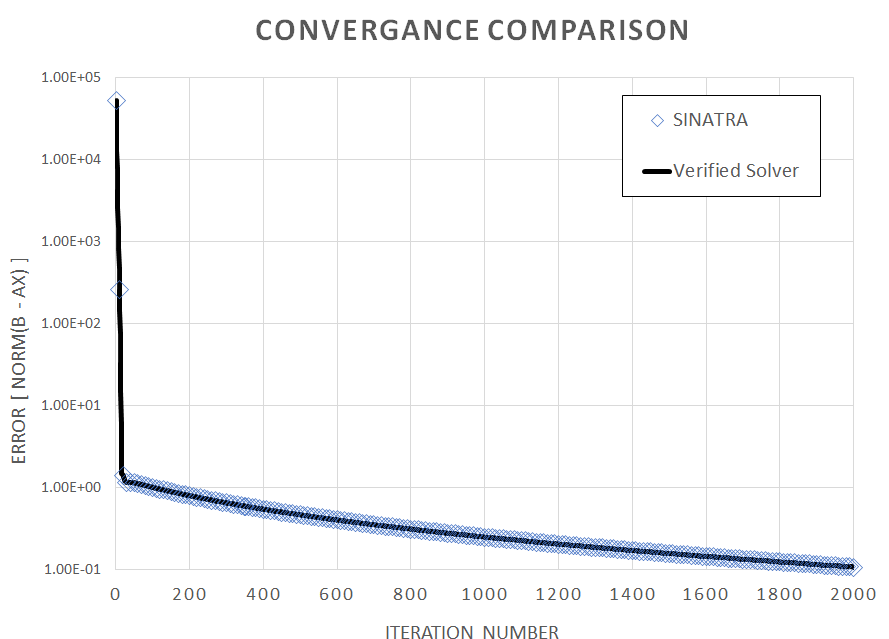
\includegraphics[width=.85\textwidth]{figures/convergance.png}
\centering
\caption[Convergence Visualization]{Error of the Gauss-Seidel solver over 2000 iterations compared to a MATLAB\textsuperscript{\textregistered} verified solver. The error is calculated through the vector norm of the difference between the stencil times the electric potential and the charge density. }
\label{fig:error64}
\end{figure}

\indent A visual way to confirm that the solver works is by observing the error as the iterations increase. A few tests were run, and the error of the solver was outputted at each iteration. A 64-cell convergence comparison is shown in Figure \ref{fig:error64}, with an average 24.8 particles per cell. It was compared to the validated solver's error residual and they are shown to match exactly. As seen in the figure, the error drops quickly and then slowly decreases towards zero. This shows numerical stability and convergence. However, it also shows that Gauss-Seidel, while robust, is not optimal for very large simulations. A visualization of the error is a good way to estimate the accuracy of the solution and just as importantly, the soundness of the initial conditions. 

\begin{table}
\caption{The initial conditions for solver verification}
\vspace{0.3cm}
\begin{tabular}{|ll|ll|}
\hline
Property               & Value                & Property                    & Value                \\ \hline
Number of Cells        & 64                 & Real to Simulated particles & \(1 \times 10^{19}\)    \\
Sphere Model           & Hard Sphere          & Collision Scheme            & Off                  \\
Time-step (s)          & \(1 \times 10^{-8}\) & Total Simulation  Time (s)  & \(5 \times 10^{-8}\) \\
Number Density         & \(1 \times 10^{24}\) & Gas Type                    & Nitrogen                \\
Electron Density       & \(1 \times 10^{12}\) & Electron Temp (eV)          & 1                  \\
Reference Potential (V)       & 0 & Domain size (m)          & \(1\times 1 \times 1\)                  \\
Stream Temperature (K) & 300                 & X,Y,Z Velocity (m/s)              & 0,0,0 \\ \hline
\end{tabular}
\label{tab:gausstable}

\end{table}

\subsection{Ambipolar Test Case}

Two main test cases were performed in order to test the validation of the SINATRA: Ambipolar diffusion and steady state electric flow. Ambipolar diffusion is a typical simulation case for PIC codes. Normal fluids will diffuse out of a domain naturally over time. However, on account of the different speeds between electrons and ions in a plasma, a gradient is set up as the electrons start to move faster than the ions. This gradient causes an electric field which in turn reduces the speed of the electrons while increasing the speed of the ions. This causes a uniform diffusion rate.  \par


\indent The initial conditions for the ambipolar diffusion were based on diffuse hot plasma consisting of argon gas \cite{plasma_table}. They can be seen in Table \ref{tab:initialambipolar}. These conditions were chosen by taking the density and temperature of a diffuse hot plasma, then calculating the other parameters according to the requirements for a PIC simulation. The Debye length was calculated to be 0.074 meters. The cell density was selected such that the cell size was approximately the Debye length. The time-step was calculated to be on the order of \(1\times 10^{-7}\) seconds and the total simulation time was chosen to see significant change in the simulation. The domain was initialized with uniformly distributed particles. The number of particles per cell was 0.85 which should be increased in future simulations for greater accuracy and to avoid numerical heating. \par

\begin{table}
\caption{The initial conditions for ambipolar diffusion}
\vspace{0.3cm}
\begin{tabular}{|ll|ll|}
\hline
Property               & Value                & Property                    & Value                \\ \hline
Number of Cells        & 4096                 & Real to Simulated particles & \(1 \times 10^9\)    \\
Sphere Model           & Hard Sphere          & Collision Scheme            & Off                  \\
Time-step (s)          & \(1 \times 10^{-7}\) & Total Simulation  Time (s)  & \(5 \times 10^{-5}\) \\
Number Density         & \(1 \times 10^{12}\) & Gas Type                    & Argon                \\
Electron Density       & \(1 \times 10^{12}\) & Electron Temp (eV)          & 100                  \\
Reference Potential (V)       & 0 & Domain size (m)          & \(1\times 1 \times 1\)                  \\
Stream Temperature (K) & 5000                 & X,Y,Z Velocity (m/s)              & 0,0,0 \\ \hline
\end{tabular}
\label{tab:initialambipolar}

\end{table}

\indent There are two simple ways to confirm that the ambipolar diffusion is working correctly. First is by comparing the density distribution throughout the simulation time. This is done through viewing a slice of the density distribution once every \(2\times 10^{-5}\) seconds. These can be seen in the full-page Figures \ref{fig:neutraldiff} and \ref{fig:ambidiff}. They are a clear validation of the implementation of the PIC simulation. In the neutral particles, it can be seen that the density near the walls slowly decreases. The sections of high density particles become smaller as more particles leave the domain. However, the charged particles are attracted to each other and join together in the middle to form a high density core of the domain. This slows the diffusion rate significantly. \par


\begin{figure}
    \centering
    \quad
  \begin{minipage}[b]{0.45\textwidth}
    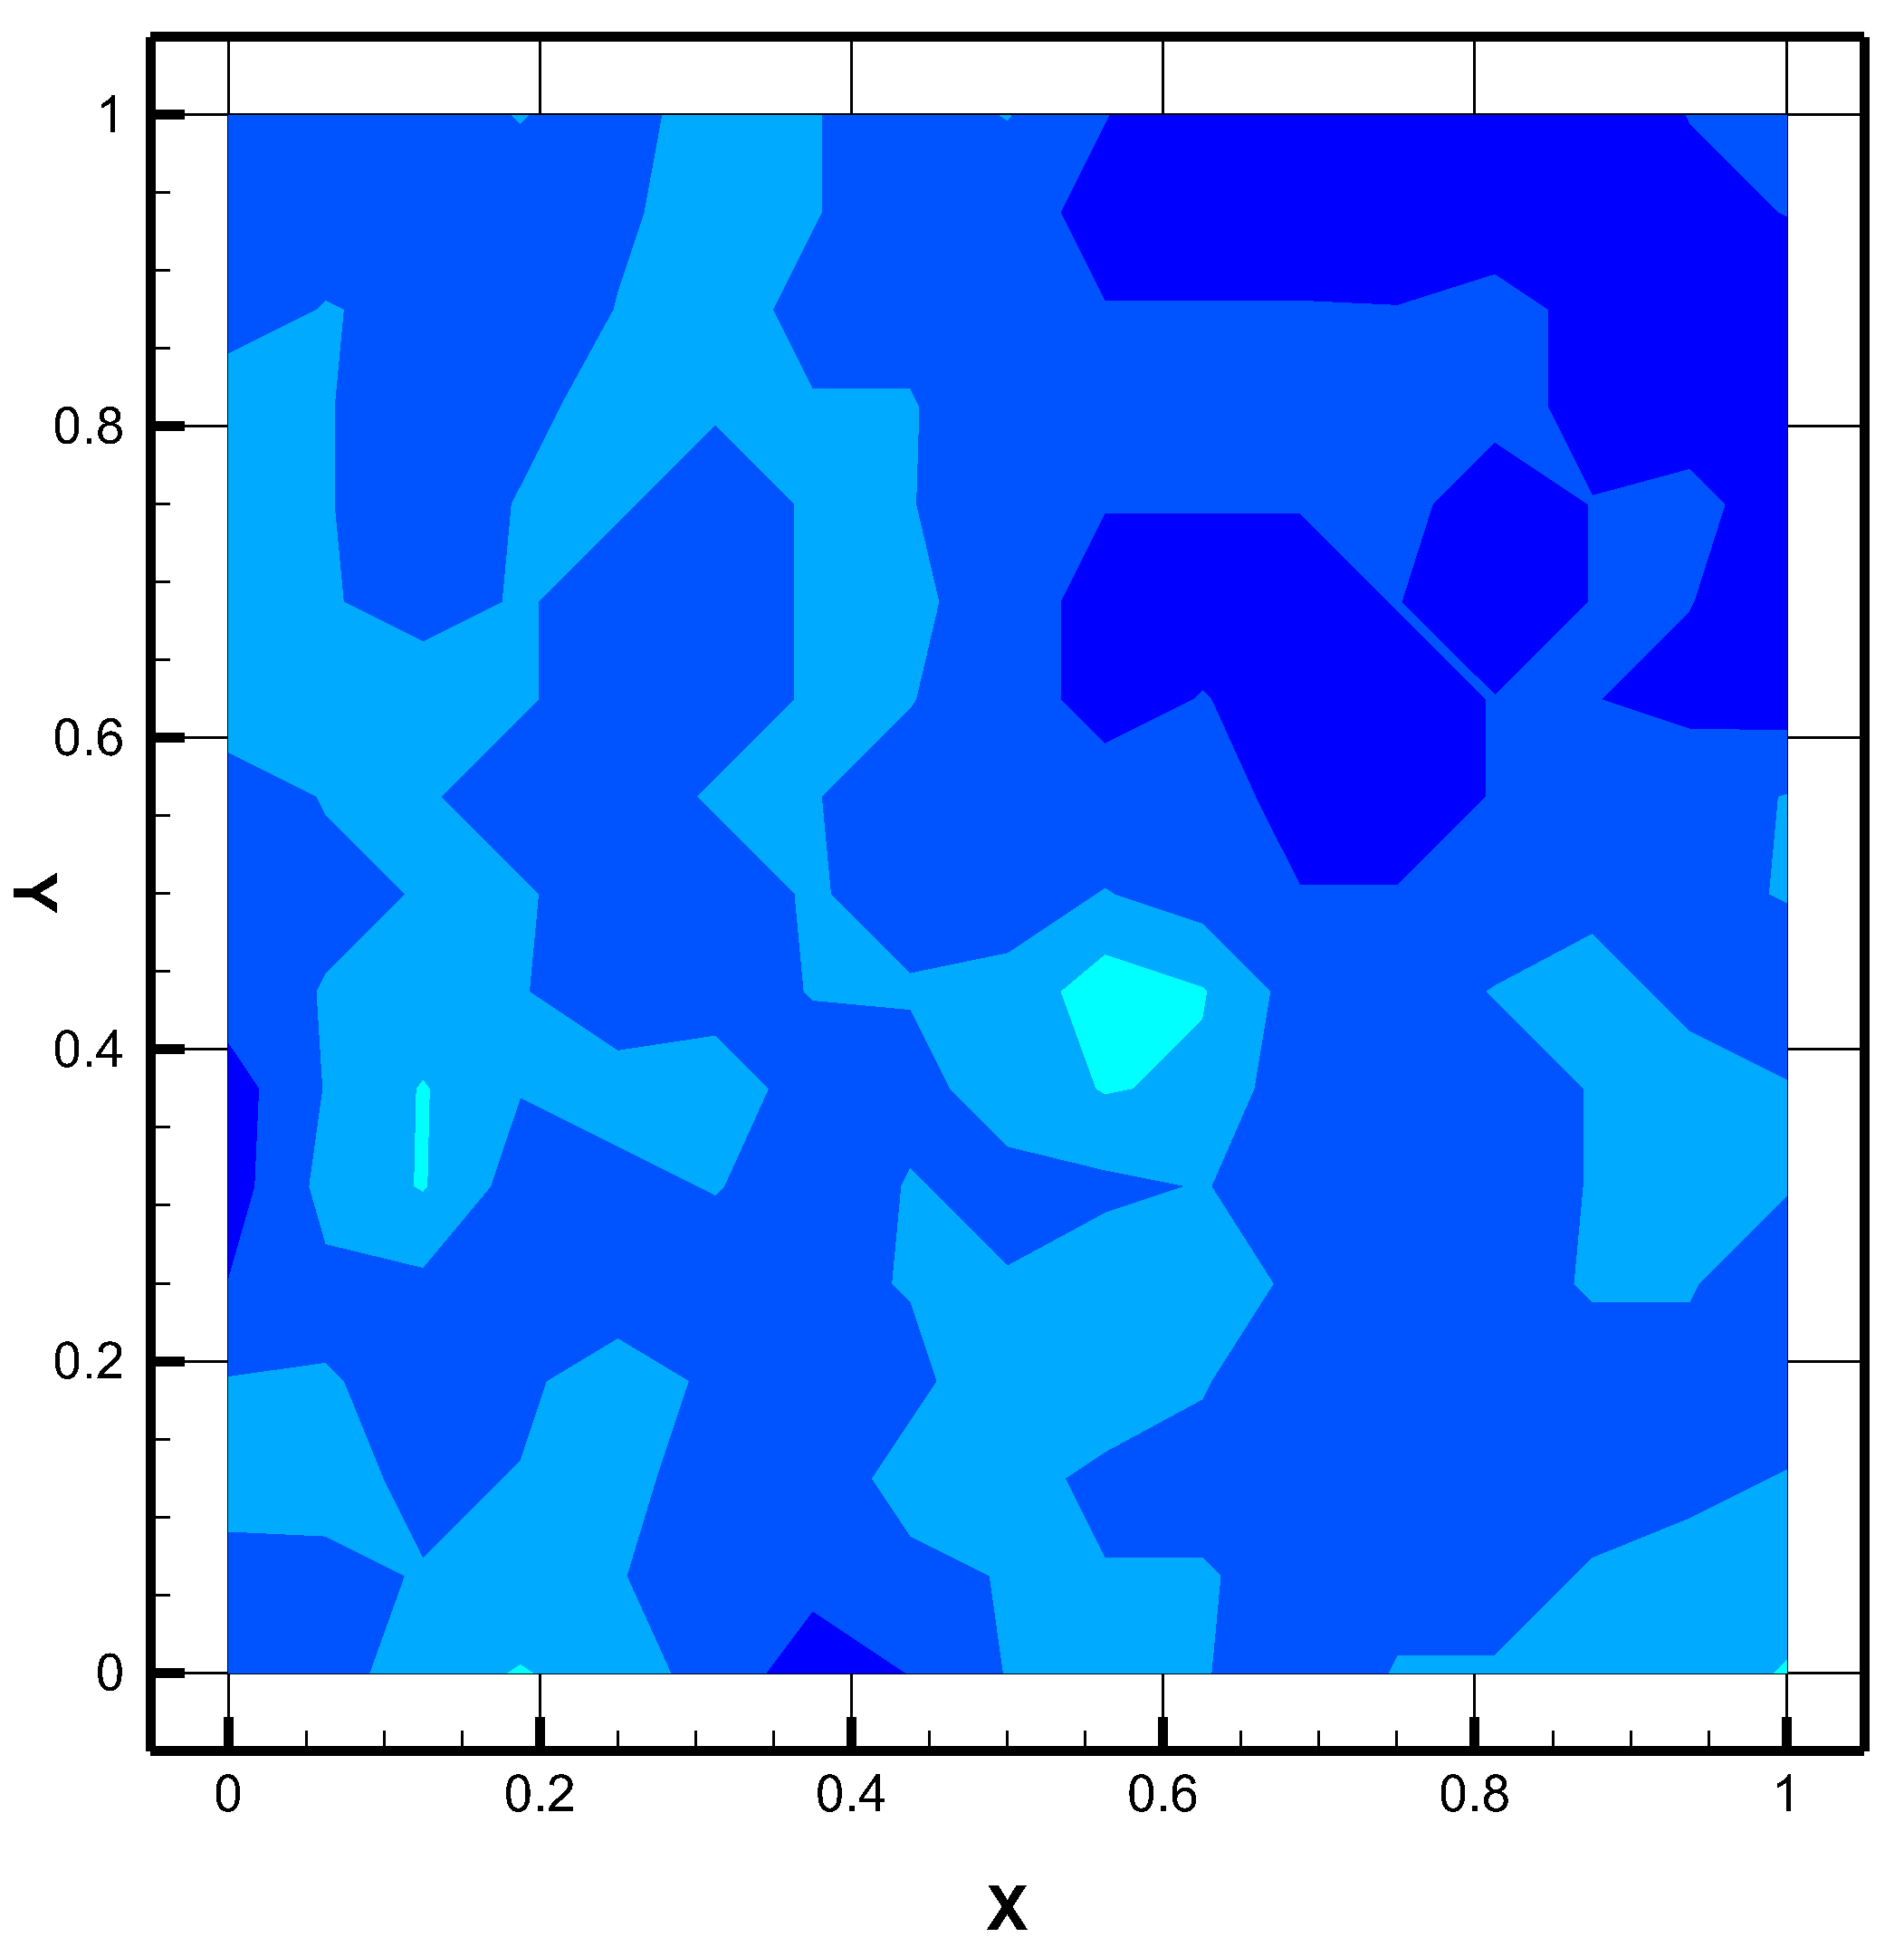
\includegraphics[width=\textwidth]{figures/Neutral1.png}
  \end{minipage} %
  \begin{minipage}[b]{0.45\textwidth}
    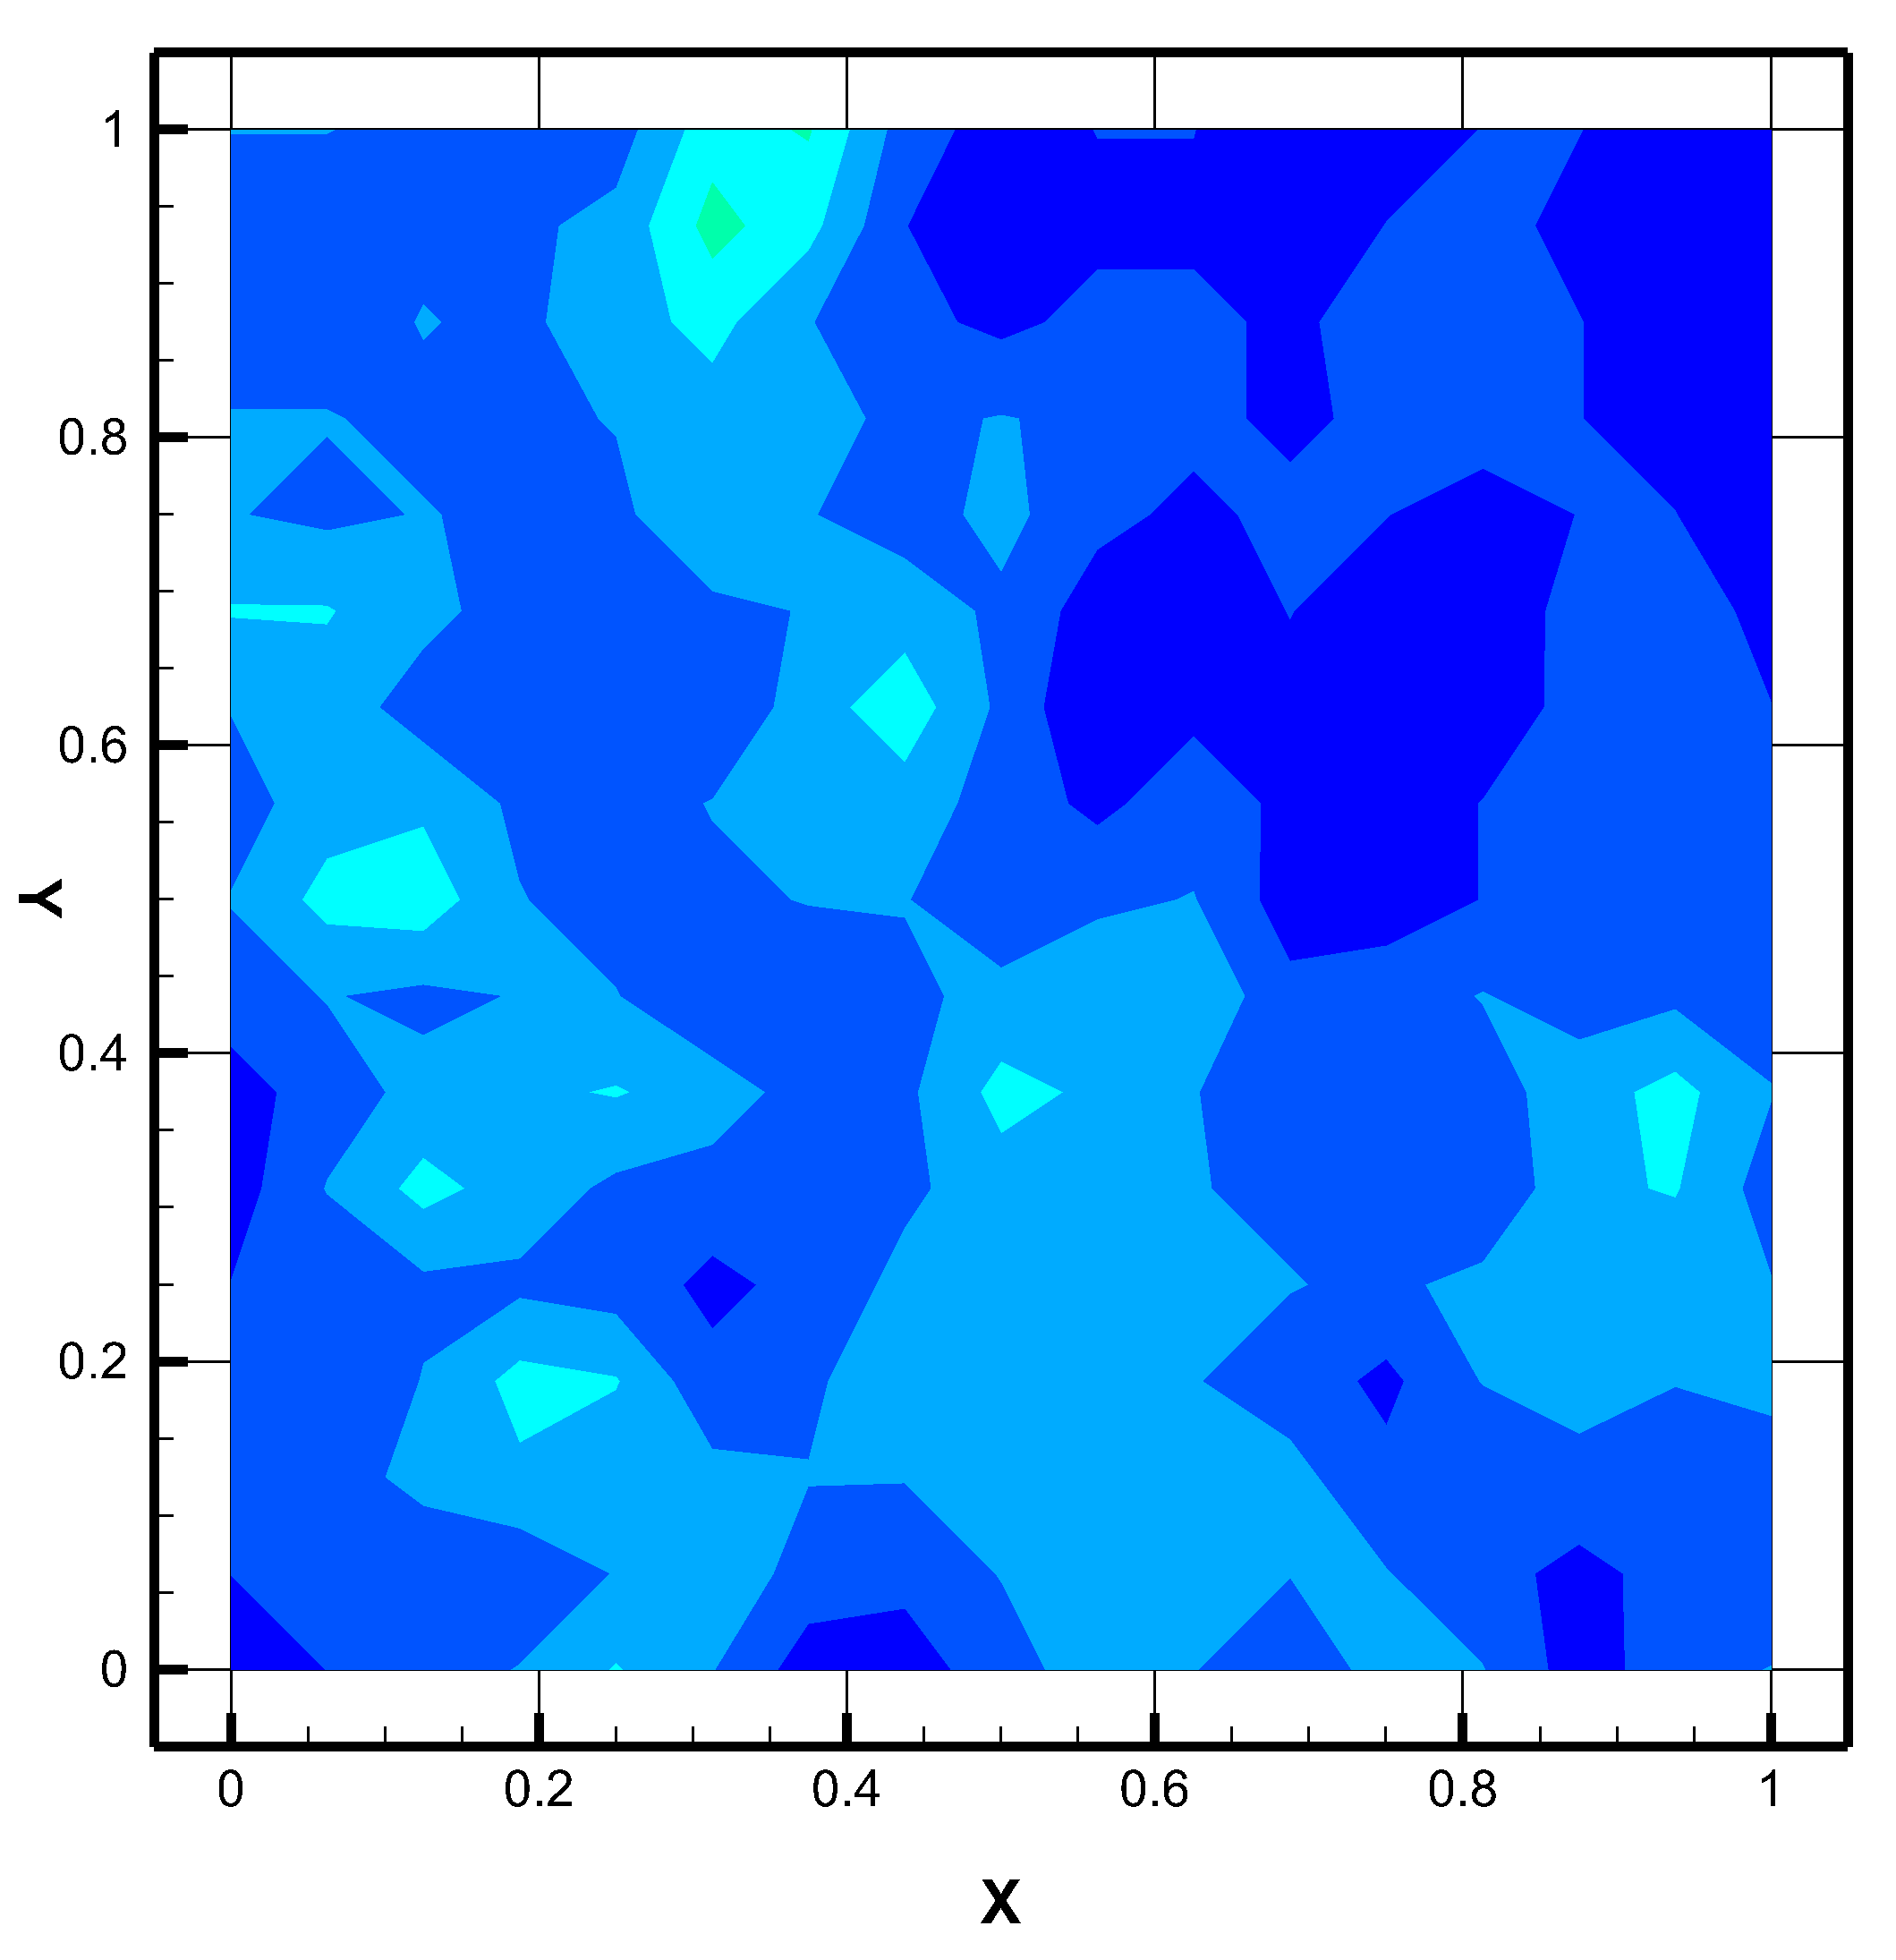
\includegraphics[width=\textwidth]{figures/Neutral2.png}
  \end{minipage} %
  \begin{minipage}[b]{0.45\textwidth}
    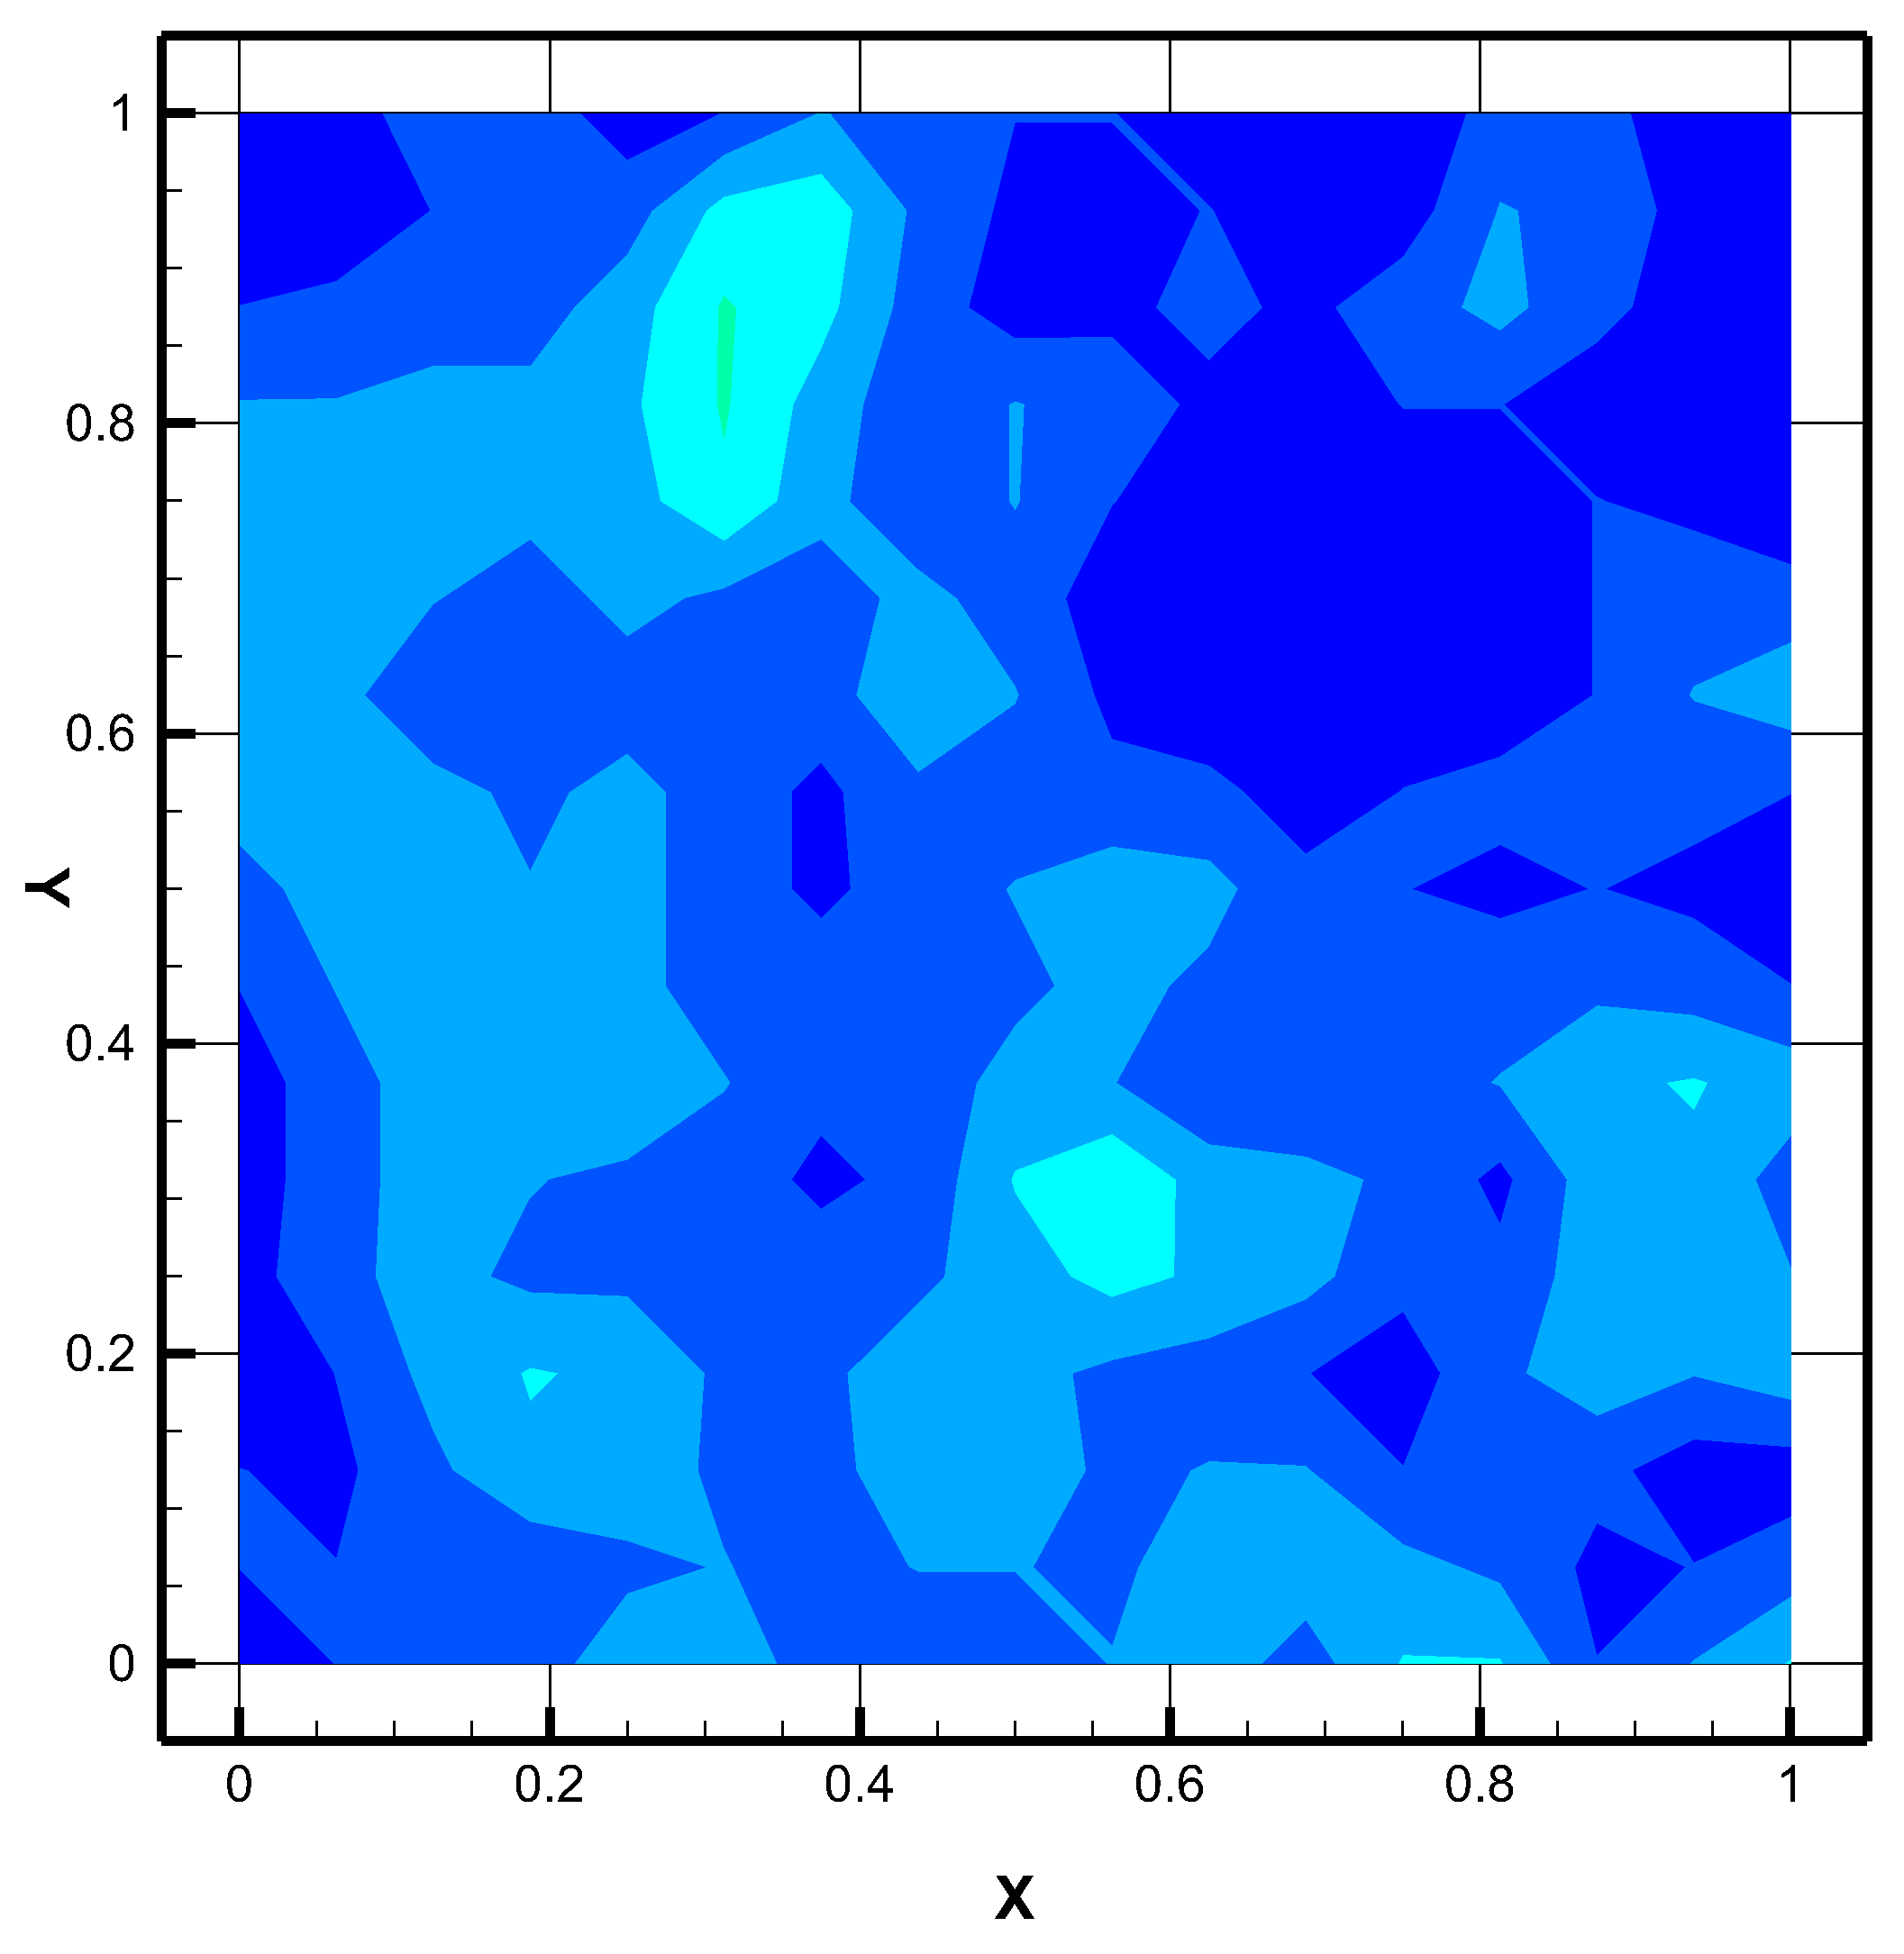
\includegraphics[width=\textwidth]{figures/Neutral3.png}
  \end{minipage} %
  \hspace{3cm}
  \begin{minipage}[b]{0.2\textwidth}
    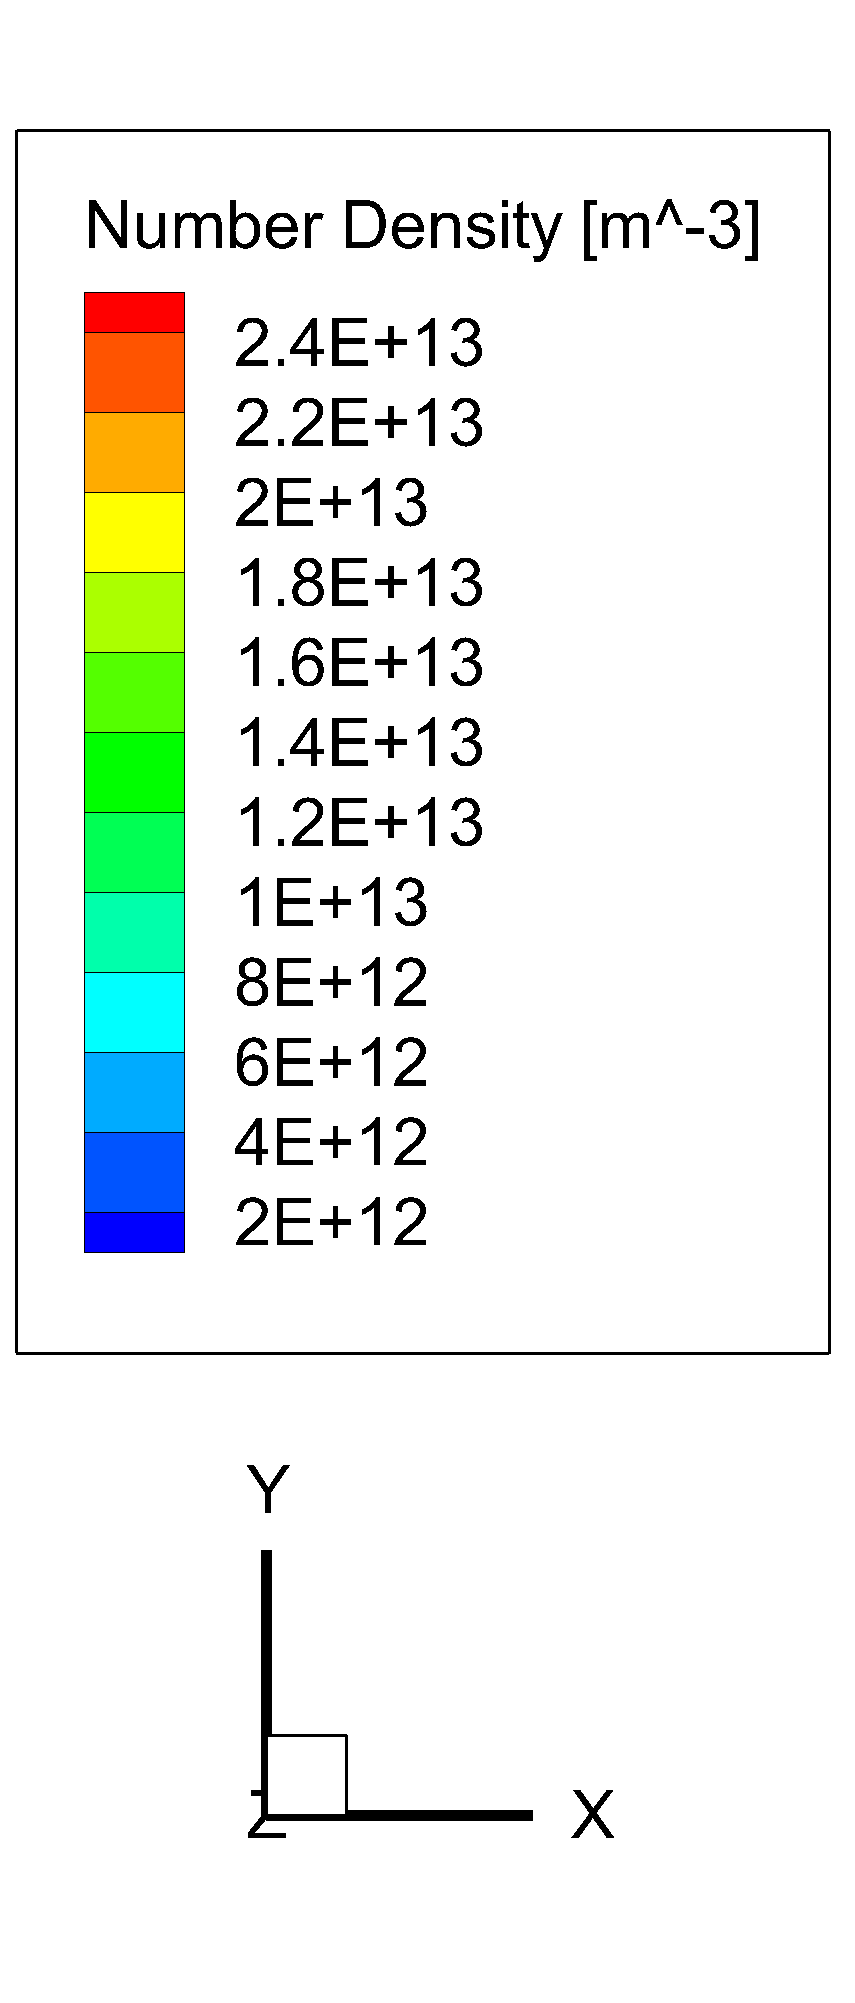
\includegraphics[width=\textwidth]{figures/legend.png}
  \end{minipage}
  \caption[Neutral Diffusion Density]{The domain of neutral diffusion from \(1\times10^{-5}\) to \(5\times10^{-5}\) seconds. First is top left, then top right, and finally bottom left. This is one slice in the Z direction as indicated by the axis, and the density levels are shown in the bottom right.}
  \label{fig:neutraldiff}
\end{figure}


\begin{figure}
    \centering
    \quad
  \begin{minipage}[b]{0.45\textwidth}
    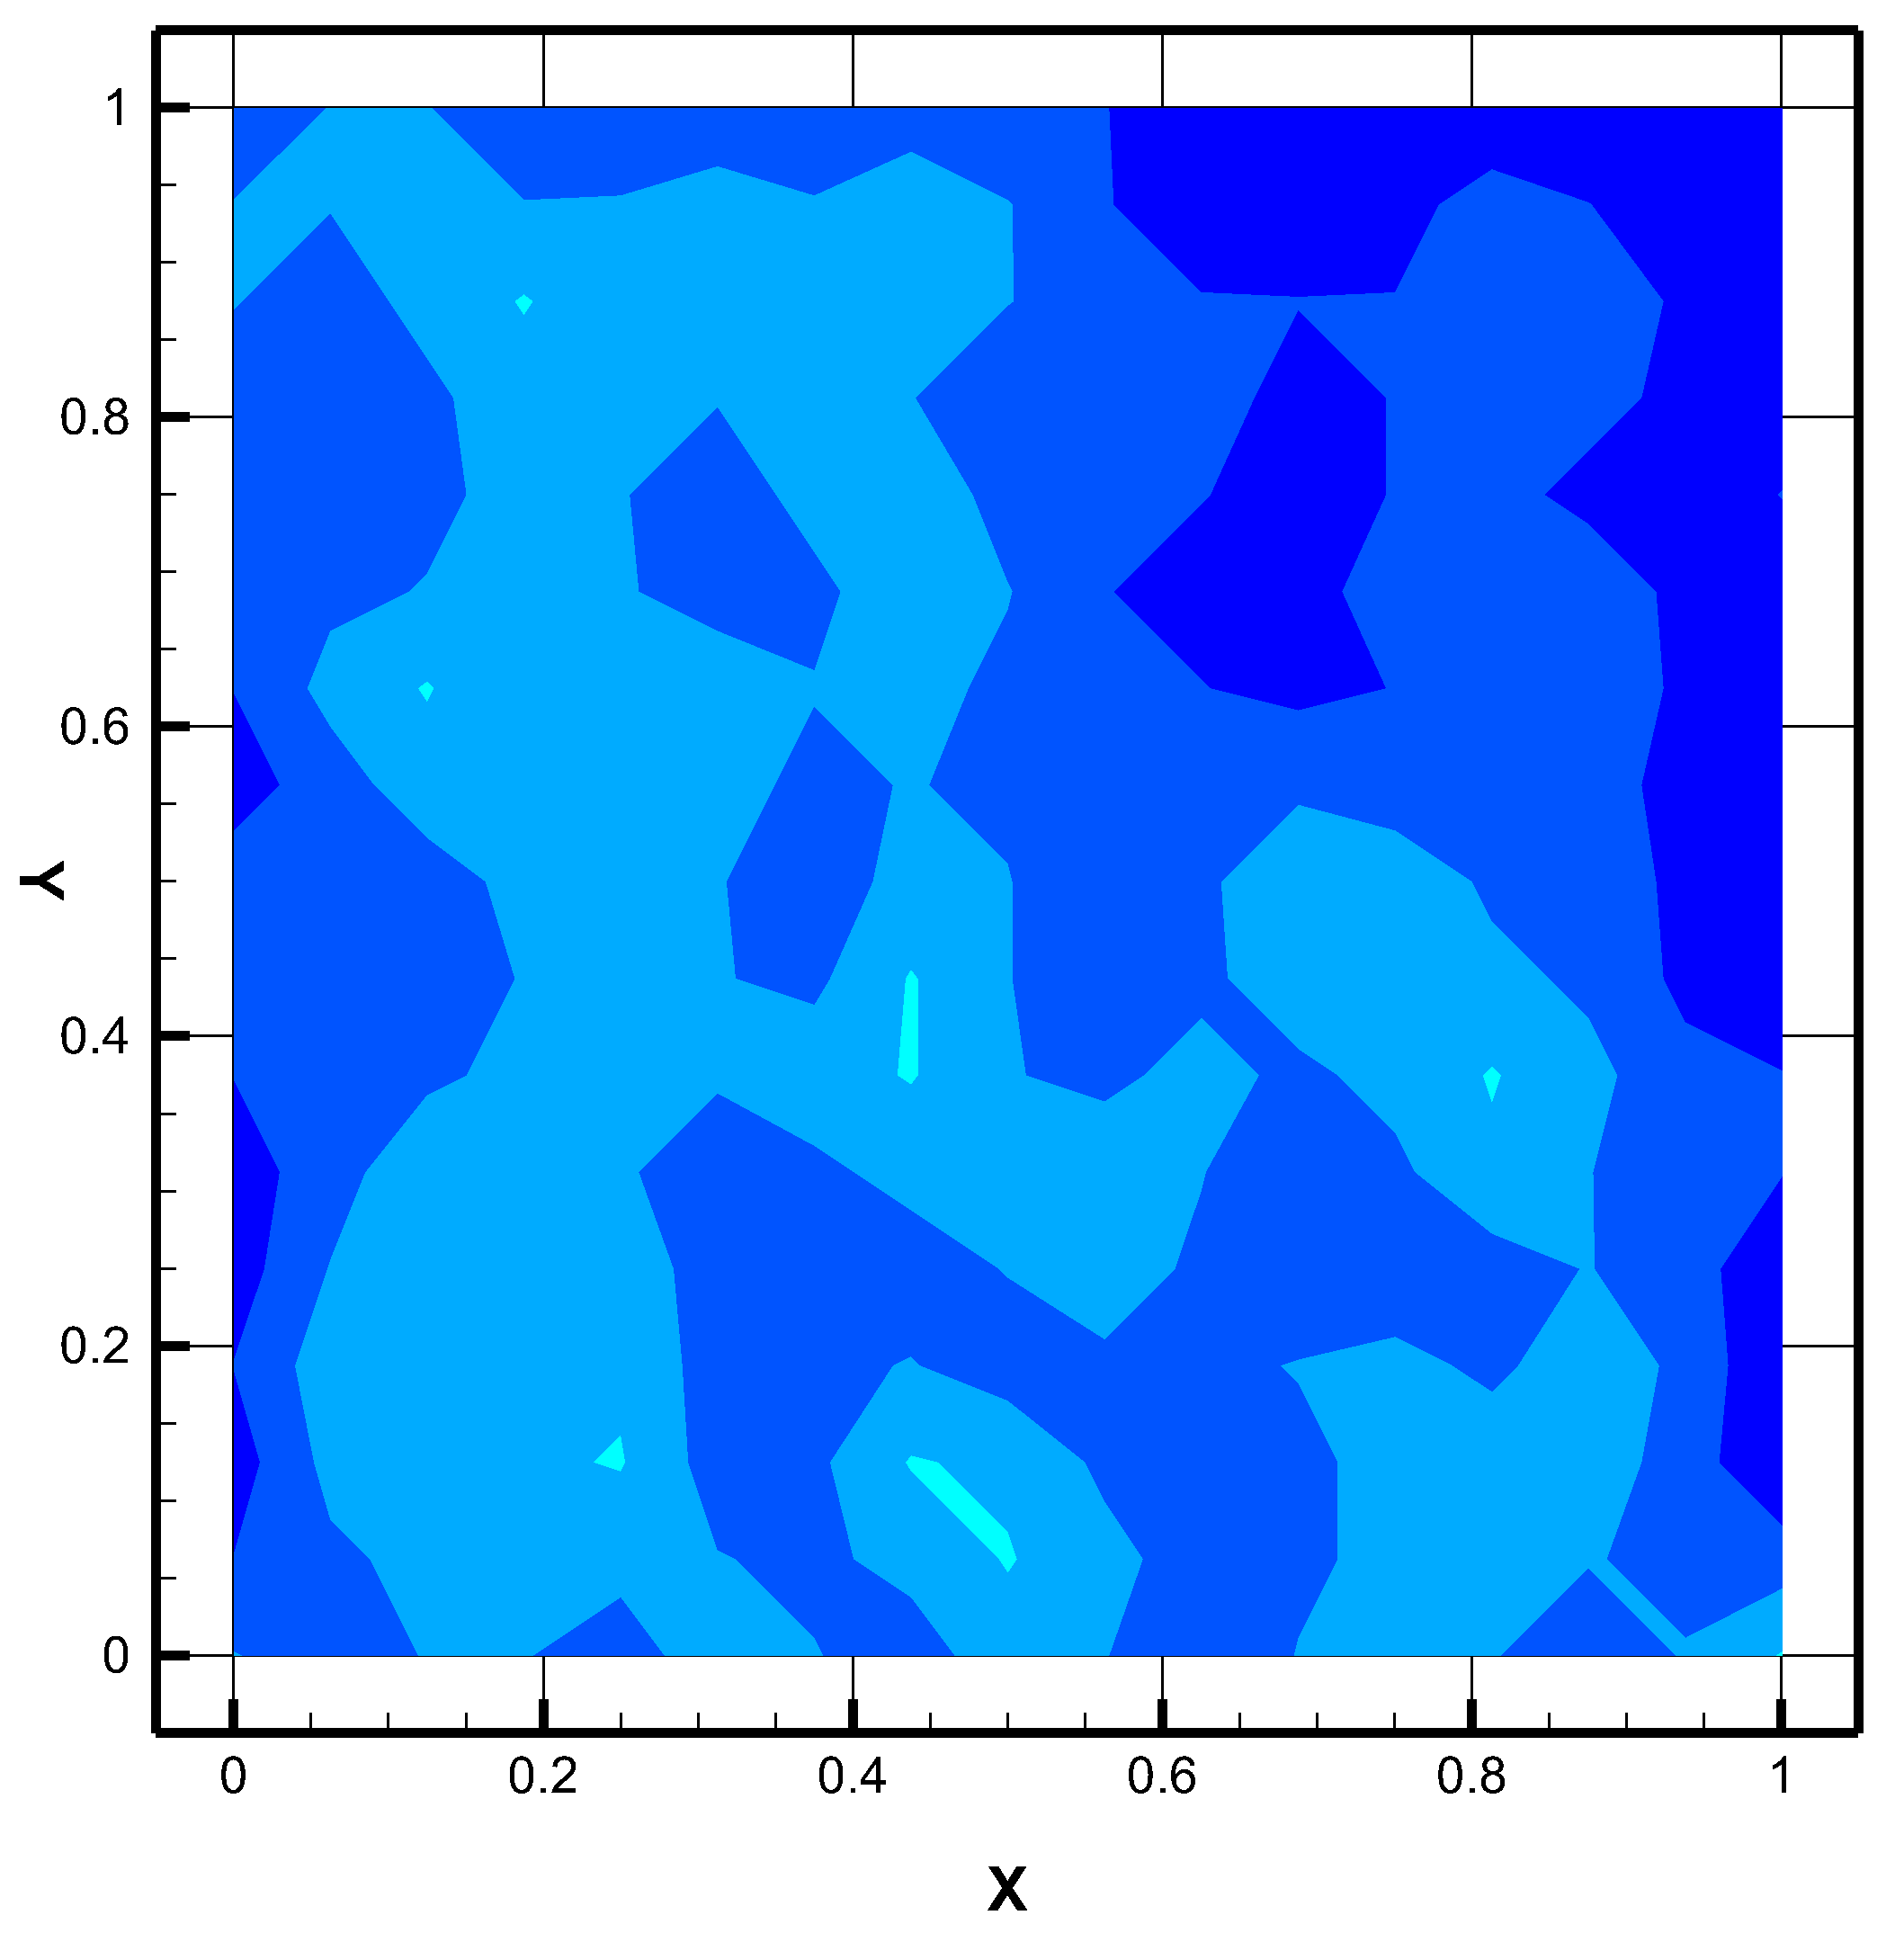
\includegraphics[width=\textwidth]{figures/Ambi1.png}
  \end{minipage} %
  \begin{minipage}[b]{0.45\textwidth}
    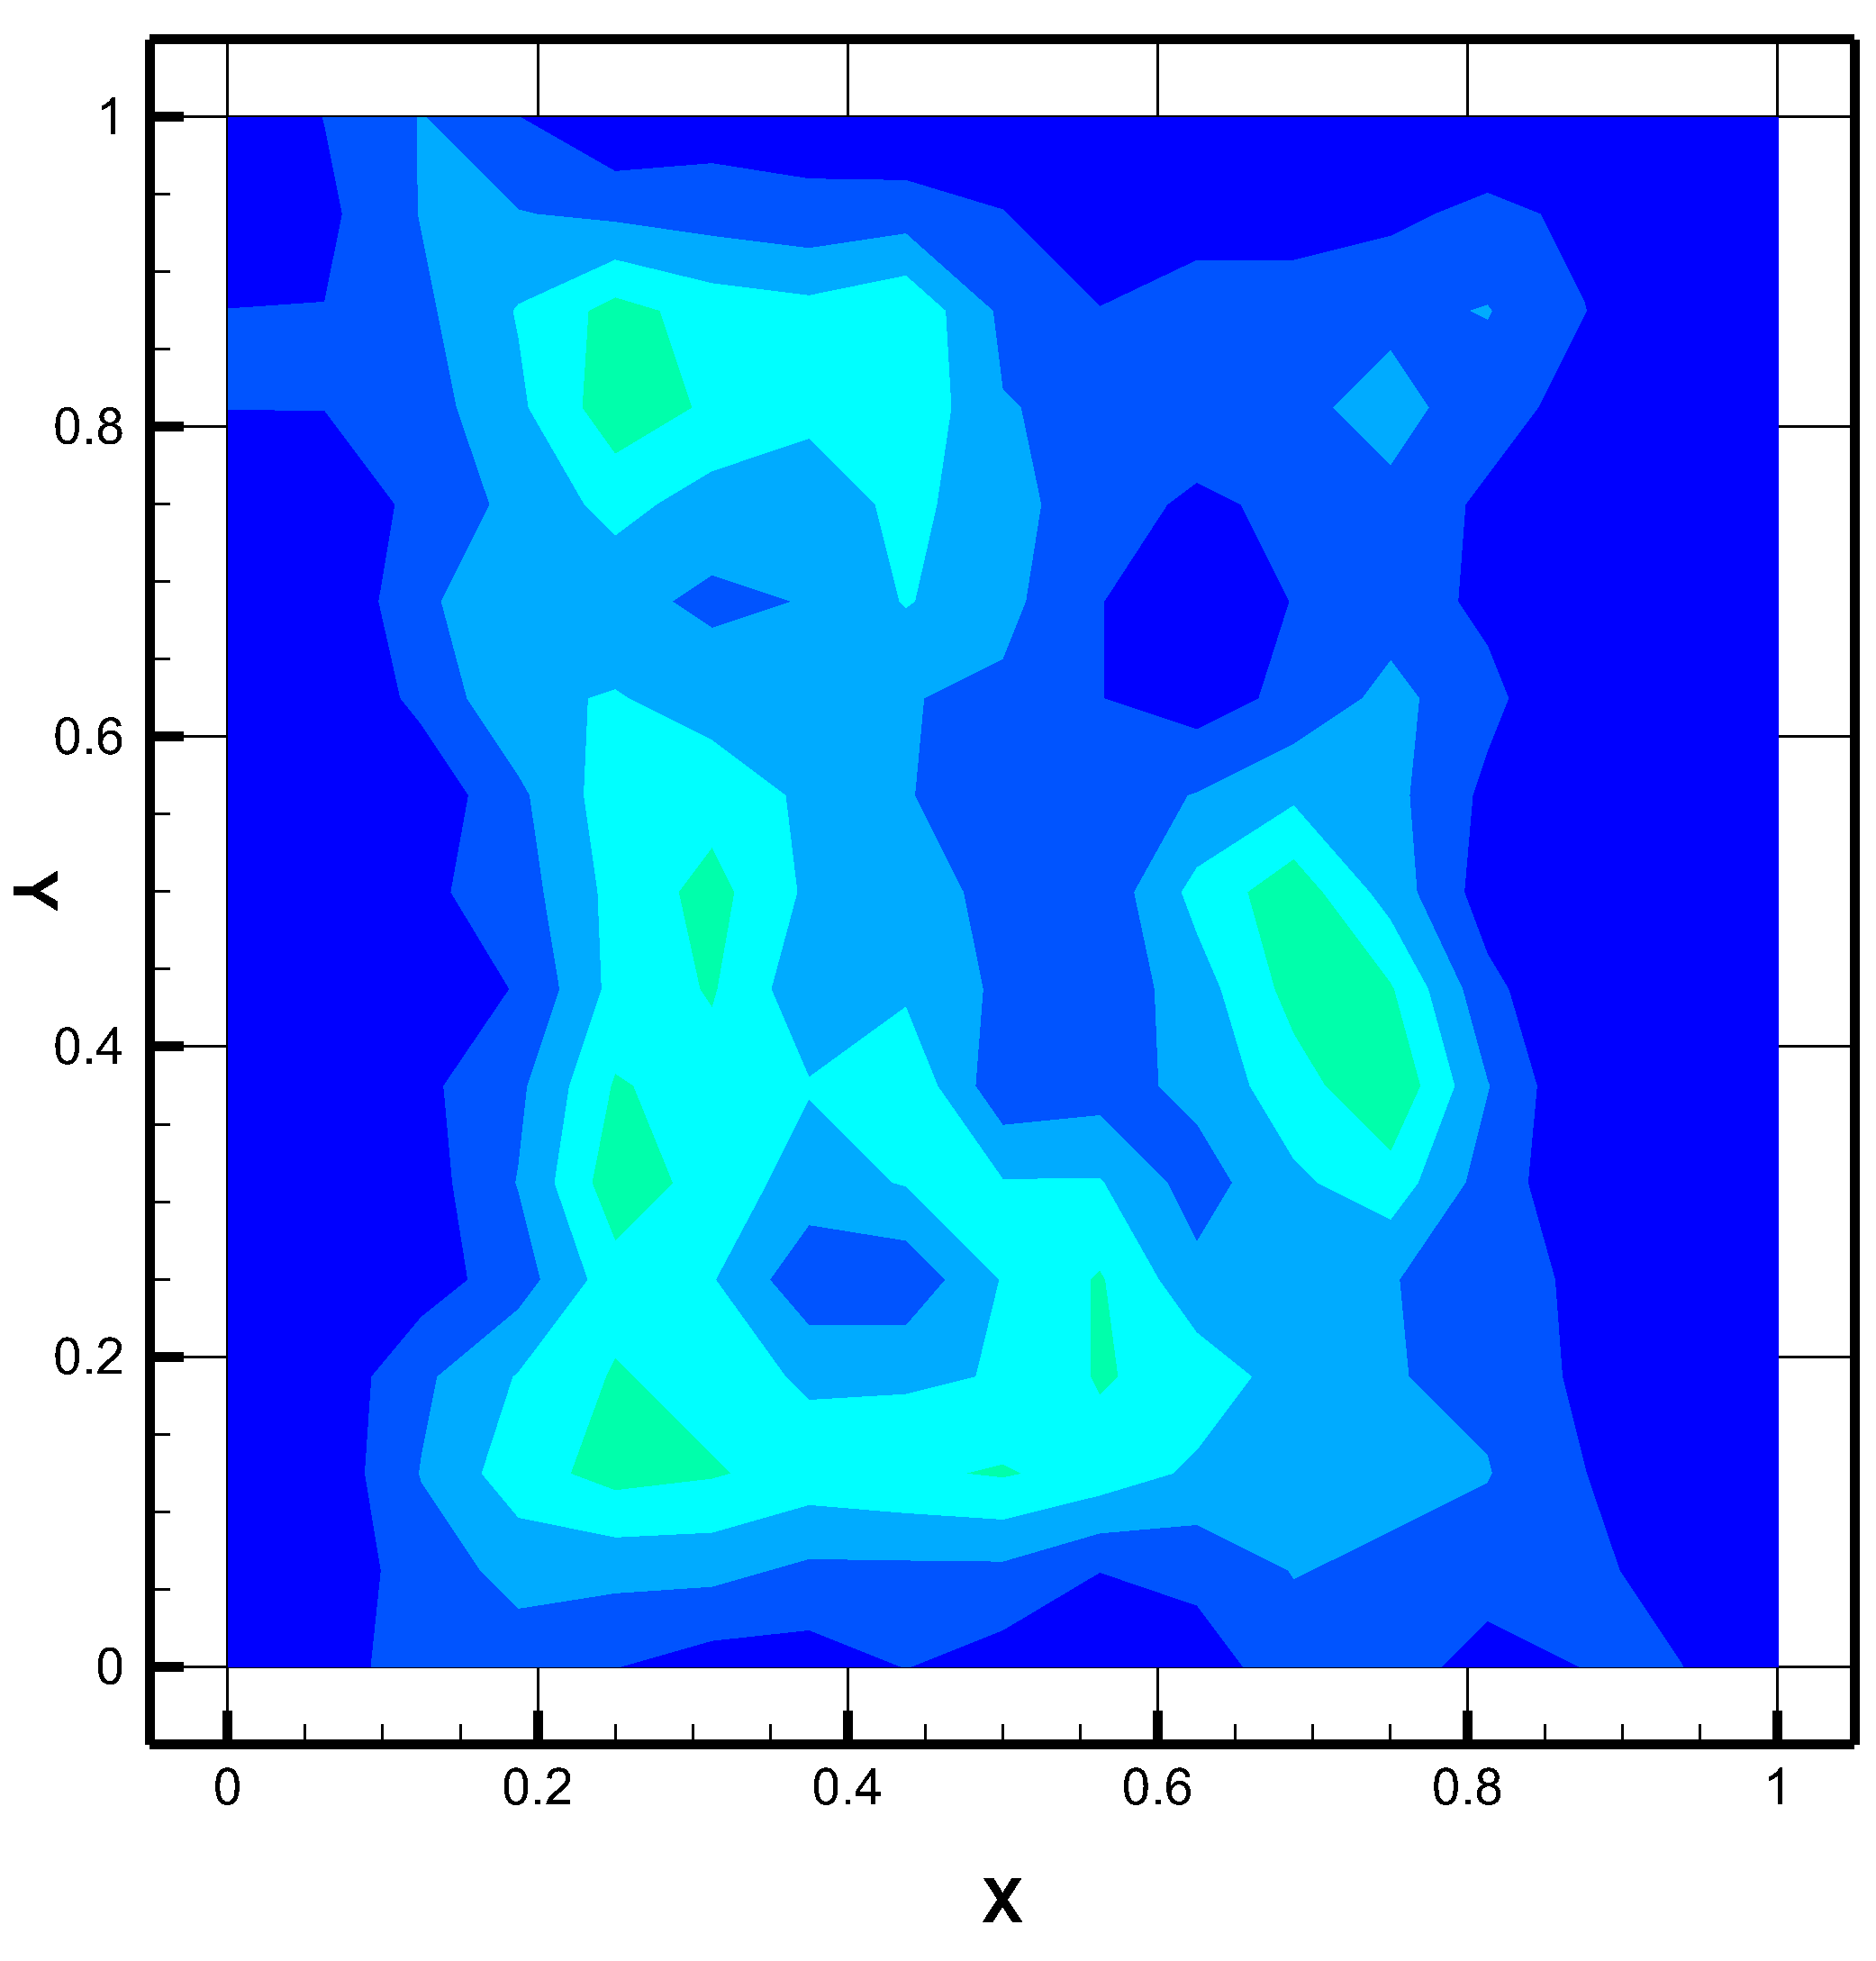
\includegraphics[width=\textwidth]{figures/Ambi2.png}
  \end{minipage} %
  \begin{minipage}[b]{0.45\textwidth}
    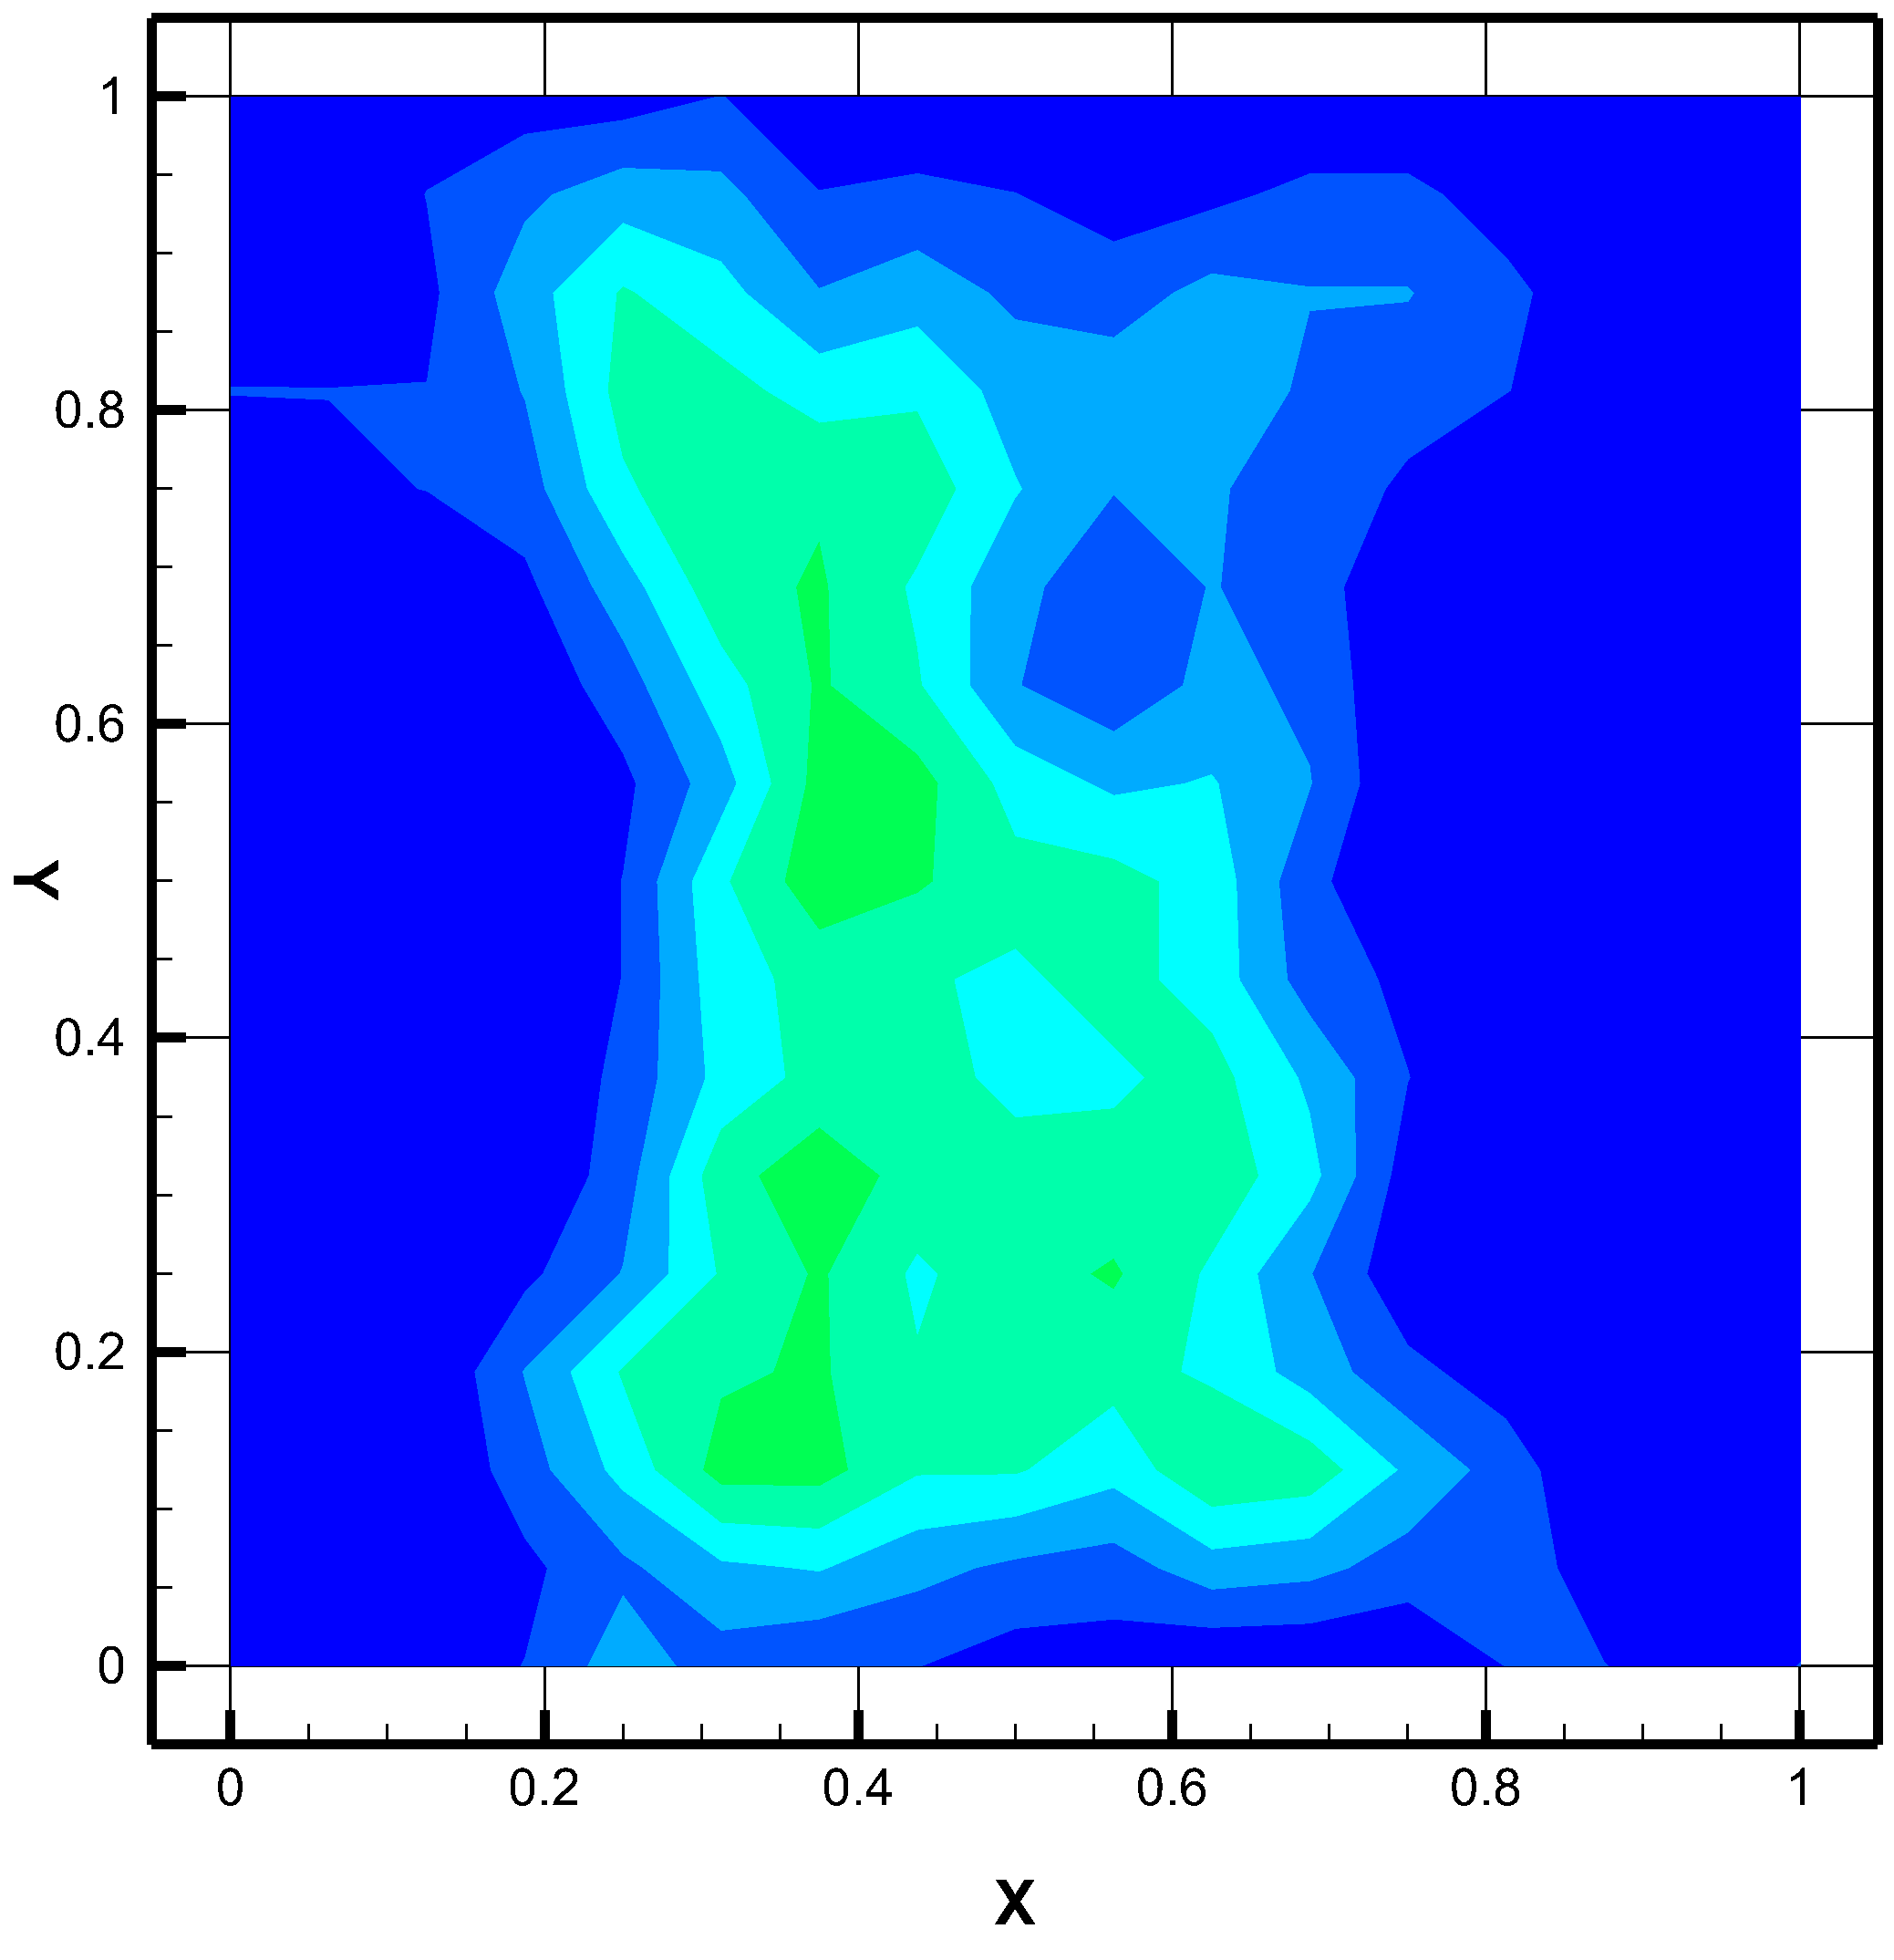
\includegraphics[width=\textwidth]{figures/Ambi3.png}
  \end{minipage} %
  \hspace{3cm}
  \begin{minipage}[b]{0.2\textwidth}
    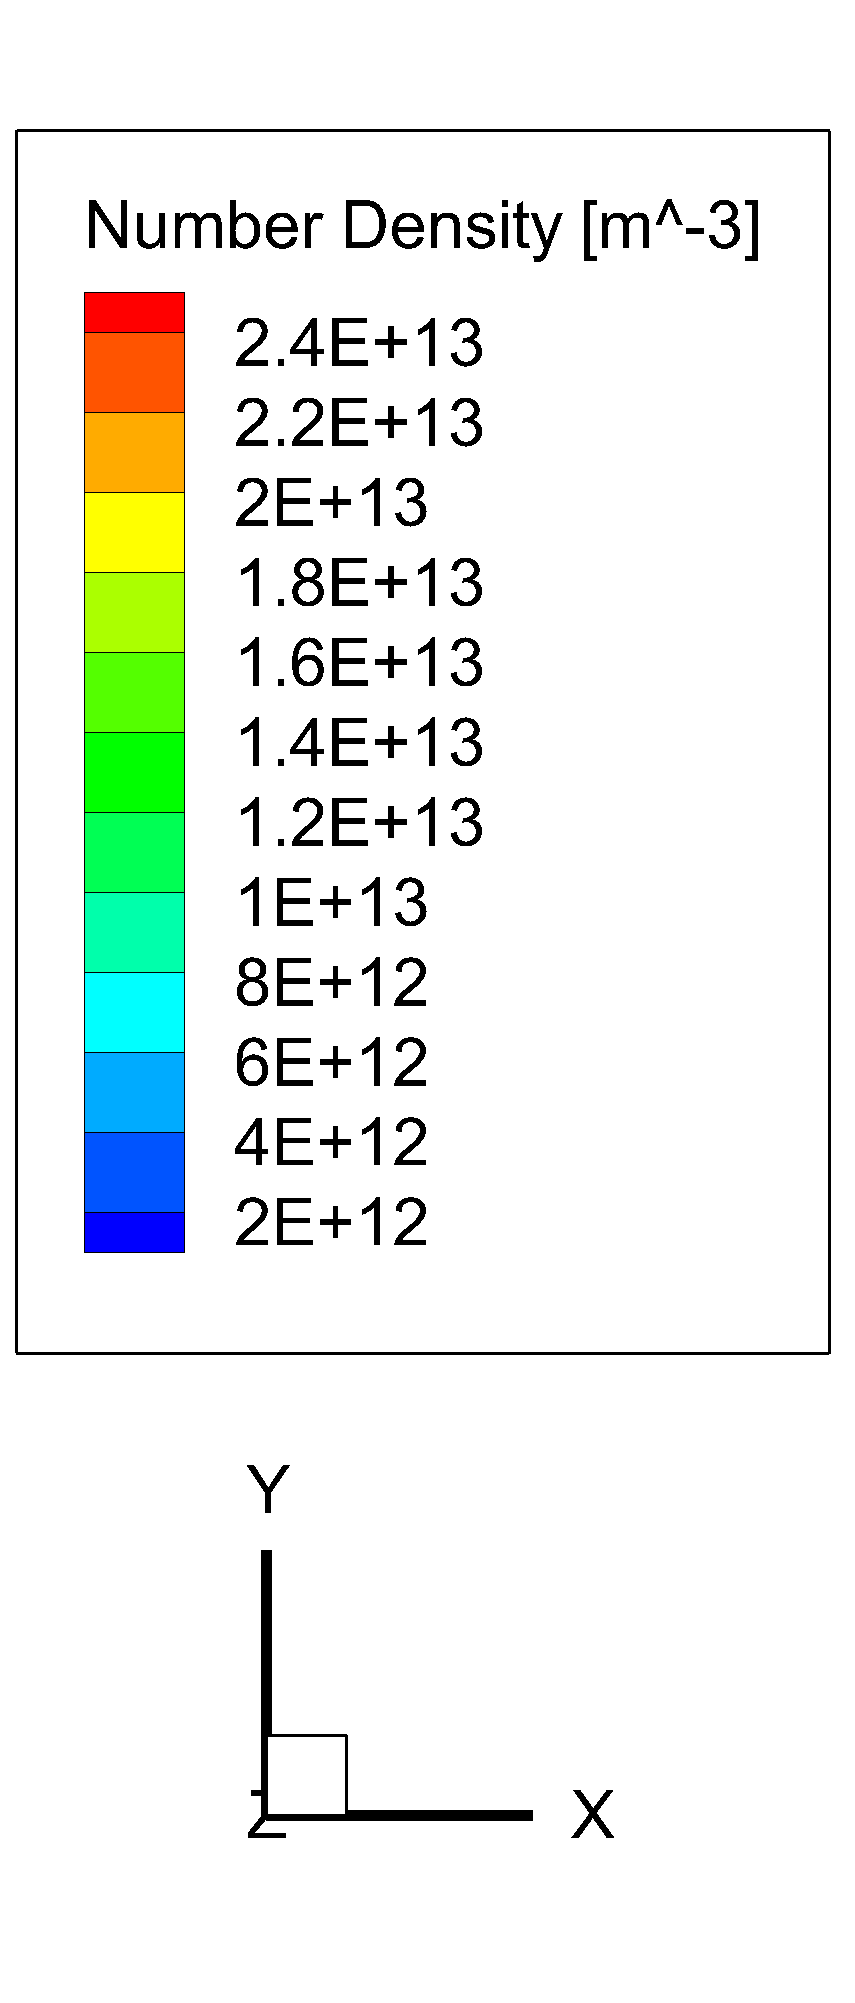
\includegraphics[width=\textwidth]{figures/legend.png}
  \end{minipage}
  \caption[Ambipolar Diffusion Density]{The domain of ambipolar diffusion from \(1\times10^{-5}\) to \(5\times10^{-5}\). First is top left, then top right, and finally bottom left. This is one slice in the Z direction as indicated by the axis, and the density levels are shown in the bottom right.}
  \label{fig:ambidiff}
\end{figure}


\indent Another metric to see if the diffusion is working is the number of particles in the domain. The number of particles is shown in Figure \ref{fig:ambipolarexcel}, and it shows the large difference between charged particles and neutrals. Both simulations begin with losing particles at a similar rate. However, within \(0.5 \times 10^{-5}\) seconds they diverge. The diffusion of the neutrals through the boundaries is relatively quick compared to the diffusion of the charge particles. Through the relative difference ambipolar diffusion can be observed. \par

\begin{figure}
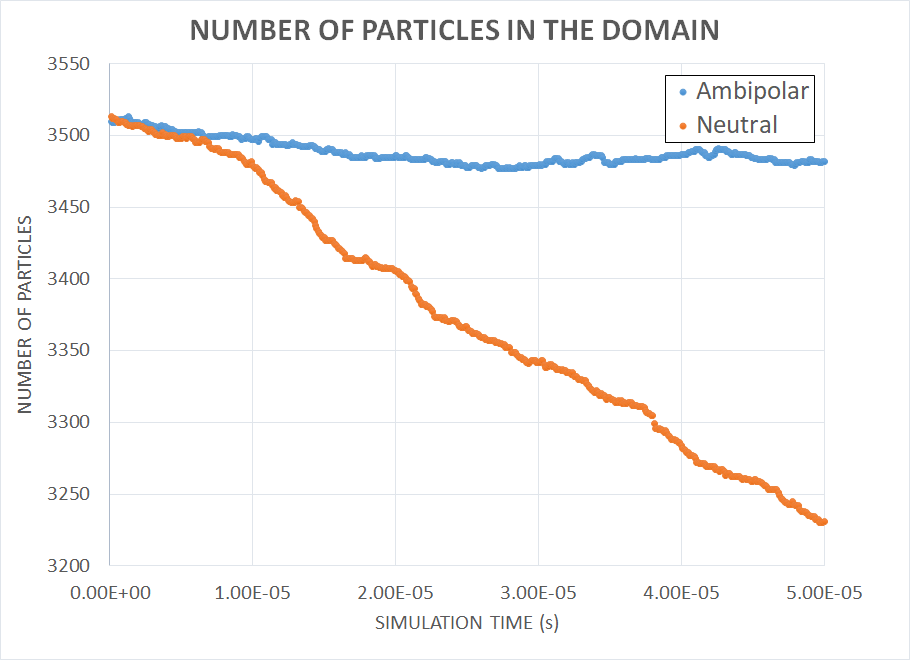
\includegraphics[width=.85\textwidth]{figures/num_particles.png}
\centering
\caption[Number of Particles in Diffusion]{The number of particles in the domain for ambipolar diffusion vs neutral diffusion}
\label{fig:ambipolarexcel}
\end{figure}

\indent Finally, an analytical comparison is a strong validation tool for the PIC implementation. For this, the ion flux can be compared to the gradient of the density because they are proportionally related \cite{gobel}. They are related by the negative ambipolar diffusion coefficient, which is shown in Equation \ref{eqn:adc}. \par

\begin{table}
\caption{Ambipolar diffusion coefficient results}
\vspace{0.3cm}
\centering
\begin{tabular}{|llllll|}
\hline
X  & Y & Z  & Flux (Y)  & Density Gradient (Y) & RHS of Eqn 4.21 (Y) \\ \hline
4  & 8 & 4  & 0.00E+00  & 0.00E+00  & 0.00E+00  \\
4  & 8 & 8  & 0.00E+00  & -2.10E+21 & 0.00E+00  \\
4  & 8 & 12 & 0.00E+00  & 0.00E+00  & 0.00E+00  \\
8  & 8 & 4  & -5.43E-07 & 2.10E+21  & 3.08E+22  \\
8  & 8 & 8  & 0.00E+00  & 0.00E+00  & 0.00E+00  \\
8  & 8 & 12 & 5.43E-07  & 0.00E+00  & -3.08E+22 \\
12 & 8 & 4  & -5.44E-07 & 0.00E+00  & 3.08E+22  \\
12 & 8 & 8  & -5.43E-07 & 0.00E+00  & 3.07E+22  \\
12 & 8 & 12 & 0.00E+00  & 0.00E+00  & 0.00E+00  \\ \hline
\end{tabular}

\label{tab:adc}

\end{table}


\Needspace{5\baselineskip}
\begin{equation}
    \label{eqn:adc}
    \tau = - D_a \nabla n 
\end{equation}
\begin{equation}
    \label{eqn:adc2}
    D_a = \frac{\mu_i D_e + \mu_e D_i}{\mu_i + \mu_e}
\end{equation}
\(\tau\) = Ion Flux \\
\(n\) = Density \\
\(D_a\) = Ambipolar diffusion coefficient\\
\(\mu\) = Ion and electron mobilities \\
\(D\) = Ion and electron diffusion coefficients \par


\indent In order to test this equation first the Ambipolar diffusion coefficient is calculated in this simulation to be \(5.6627\times10^{28} \: m^2/s\) using the code found in Appendix \ref{app:adc}. Then the gradient in a direction and the flux is calculated over test points within the domain. These were then compared and can be seen in Table \ref{tab:adc}. A few notes on these results are as follows. First, the low number of particles makes the results very discretized and therefore not consistent. Also, the ambipolar diffusion has made some cells have no particles and therefore the densities are actually 0, giving a skewed result. However, what can be seen is the magnitude of the results. This is shown to be within 1 order of magnitude. This is acceptable on account of two reasons. First, the ambipolar diffusion coefficient assumes a continuum solution and therefore is not completely accurate in this simulation. Secondly, the all neumann boundary simulation means that the simulation may find a solution which is not necessarily the most accurate solution. These two sources of error explain the error in these results. 





\subsection{Steady State Flow}

\indent An electric propulsion plume can be approximated by a simulation with all the boundaries as outflows except for a single inlet. That inlet has some initial velocity into the domain. This is the second test case for the PIC implementation into SINATRA. It serves two purposes. First, it is a starting point for a complicated electric propulsion plume. Secondly, it is a strong visual tool to confirm that the poisson equation solver is generating reasonable electric potential values. All boundaries are outflows while the -X boundary is an inlet with velocity going into the domain. Table \ref{tab:intialstead} shows the initial conditions for this test case. The domain is uniformly initialized for number of particles per cell (9.85) and given an Maxwellian distribution for velocity of 1000 m/s in the X direction. \par



\begin{figure}
    \centering
    \quad
  \begin{minipage}[b]{0.45\textwidth}
    \centering
    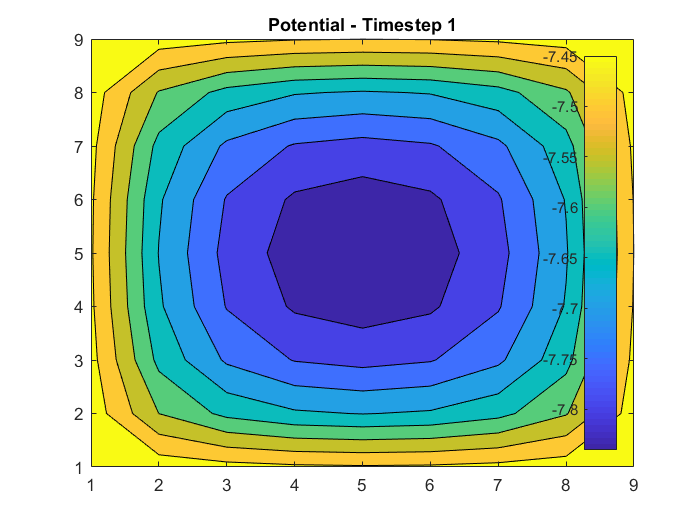
\includegraphics[width=\linewidth]{figures/potential_1.png}
  \end{minipage} %
  \begin{minipage}[b]{0.45\textwidth}
    \centering
    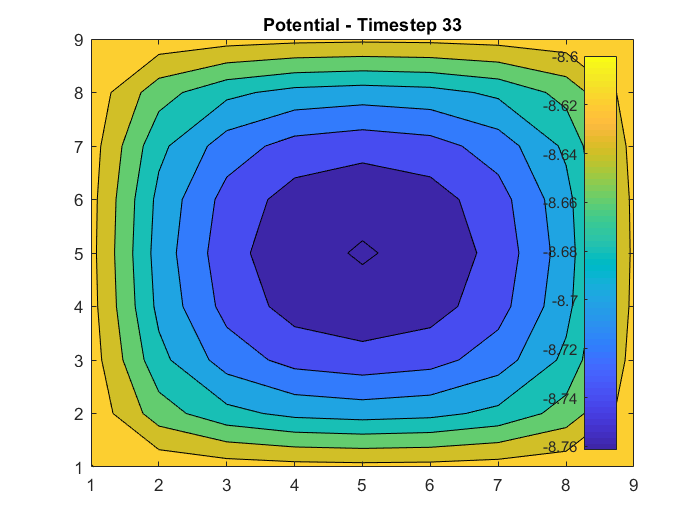
\includegraphics[width=\linewidth]{figures/potential_33.png}
  \end{minipage} %
  \begin{minipage}[b]{0.45\textwidth}
    \centering
    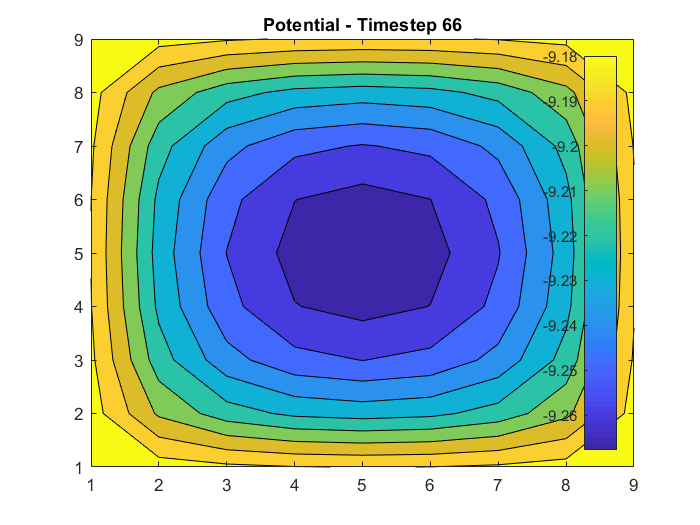
\includegraphics[width=\linewidth]{figures/potential_66.png}
  \end{minipage} %
  \begin{minipage}[b]{0.45\textwidth}
    \centering
    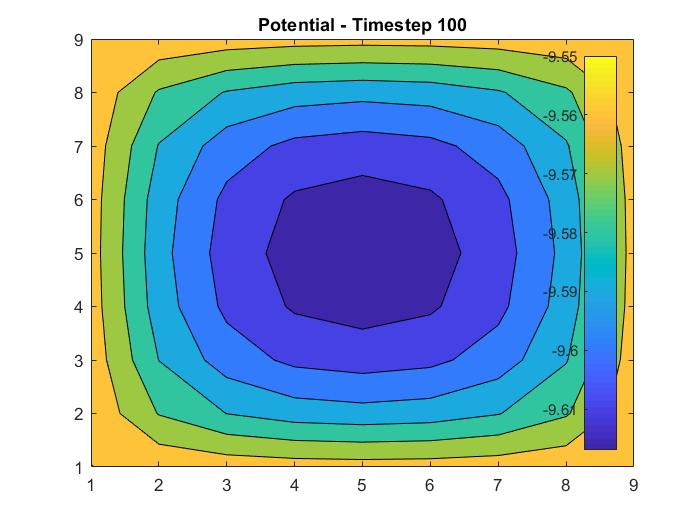
\includegraphics[width=\linewidth]{figures/potential_100.png}
  \end{minipage}
  \caption[Steady State Potential]{The domain of steady state flow from \(1\times10^{-8}\) to \(1\times10^{-6}\). First is top left, then top right, and then bottom left, and finally bottom right. This is one slice in the Z direction at node 4. The color bar shows the value of the potential.}
  \label{fig:steadypot}
\end{figure}


\begin{figure}
    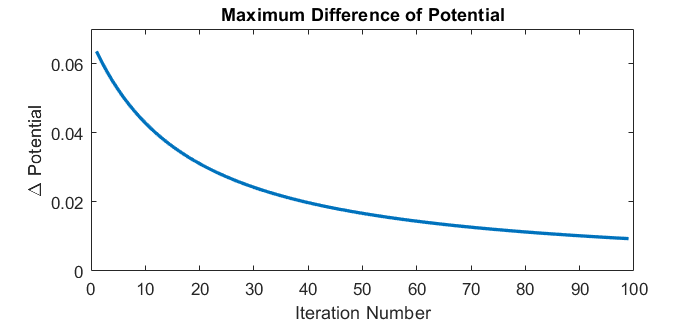
\includegraphics[width=.85\textwidth]{figures/steadyconvergance.png}
    \centering
    \caption[Maximum Difference in Potential]{The maximum difference in potential across one slice of the domain in the Z direction at node 4. The steady state convergence can be seen in the approach to 0 difference in potential.}
    \label{fig:steadyconvergance}
\end{figure}

\indent Figure \ref{fig:steadypot} shows the contours of the potential across a slice of the domain. This figure shows how the electric potential does not have any large numerical instabilities, it does not change shape dramatically between time-steps, and it is relatively regular as expected for an empty domain. To show that as time progresses the simulation is reaching the steady state solution, the maximum difference in the potential between time-steps was calculated and plotted in Figure \ref{fig:steadyconvergance}. The asymptotic nature of the difference approaching zero shows that this simulation is converging upon a steady state solution to the given initial conditions. This is not the Gauss-Seidel solver slowly converging upon a solution because the 5\% solver requirement was used which ensures that the Gauss-Seidel is steady before moving on to the next time iteration. This test case validates a correct implementation of charged particles as well as well-suited initial conditions to study complicated electric propulsion plumes. 


\begin{table}
\caption{The initial conditions for steady state flow}
\vspace{0.3cm}

\begin{tabular}{|ll|ll|}
\hline
Property               & Value                & Property                    & Value                \\ \hline
Number of Cells        & 512                  & Real to Simulated particles & \(1 \times 10^9\)    \\
Sphere Model           & Hard Sphere          & Collision Scheme            & Off                  \\
Time-step (s)          & \(1 \times 10^{-8}\) & Total Simulation  Time (s)  & \(1 \times 10^{-6}\) \\
Number Density         & \(5 \times 10^{12}\) & Gas Type                    & Argon                \\
Electron Density       & \(1 \times 10^{12}\) & Electron Temp (eV)          & 1                    \\
Reference Potential (V)       & 0 & Domain size (m)          & \(1\times 1 \times 1\)                  \\
Stream Temperature (K) & 5000                 & X,Y,Z Velocity (m/s)        & 1000,0,0             \\ \hline
\end{tabular}

\label{tab:intialstead}

\end{table}
% bad orphan





\subsection{Execution Time Study}

In order to examine the performance of SINATRA after the inclusion of PIC, an execution time study was performed. The convergence condition was tested as both the absolute error being less than 0.05 Volts and a less than a 5\% difference in the error from the last 50 iterations. Simulations were run keeping the same number of particles but changing the mesh size, as well as holding the mesh size and changing the number of particles. It is also compared to a similar non-charged simulation. The results can be found in Table \ref{tab:pic_time}.

\indent These simulations used the same settings as ambipolar diffusion. There were 2500 maximum iterations and it was run for 500 time-steps. First, the large difference (over 98\%) between the neutral simulation and similar charged particle simulations is evident. This is on account of the large number of iterations necessary to solve the electric potential. Secondly, the difference between the 5\% percent change convergence condition and the 0.05 Volts absolute error condition is significant, on the order of 65\%. This can be attributed to the fact that if a time-step does not converge, the next time-step starts where the last one ended, because electric potential is not reset between time-steps. Consequentially, the solver keeps trying to reduce the error throughout all the time-steps. In the percent change simulation, it can be seen that the first simulation reaches convergence, and the sequential time-steps only need to solve the slight difference in the charge density caused by the moving particles. However, the first iteration of the absolute error simulation takes the same amount of time as the other iterations and therefore it is continually reaching the maximum time-steps attempting to reduce the error\footnote{This was confirmed by an examination of the output logs}. \par

\begin{table}
\caption{PIC Execution Time}
\label{tab:pic_time}
\vspace{0.3cm}
\begin{center}
\begin{tabular}{|l|l|l|l|}
\hline
                             & First Iteration & Time-step Average & Total Time     \\ \hline
Neutral & 2 sec           & \(<\) 1 sec           & 3 min, 4 sec  \\ \hline
5\% error convergence   & 1 min, 56 sec   & 24 sec    & 199 min, 44 sec \\ \hline
0.05 V error convergence   & 18 min, 46 sec   &  18 min, 46 sec   &   578 min, 11 sec\tablefootnote {Extrapolated from first 25 time-steps, assuming same average up to time-step 100, then 24 seconds per time-step.} \\ \hline
64 Cells, 5\% error   & \(<\) 1 sec   & \(<\) 1 sec    & 15 sec \\ \hline
10 times more particles   & 1 sec   & \(<\) 1 sec    & 26 sec\tablefootnote {Extrapolated from 30 time-steps, errors on account of too many particles in each cell} \\ \hline

\end{tabular}
\end{center}
\end{table}

\indent Through the results in Table \ref{tab:pic_time}, it can be seen that the execution time is more heavily influenced by the number of mesh cells than the number of particles. When the number of cells is reduced to 64, the execution time is reduced from over 3 hours to 15 seconds. It follows that the combination of an octree mesh and a non-optimal code dramatically changes the simulation time. The final simulation uses a 64-cell mesh and increases the number of simulated particles by 10 times. Even with the increased number of particles there is only an 11-second difference. This shows how the number of cells has a larger influence than the number of particles. It also shows that parallization makes a negligible difference in the PIC code unless the number of simulated molecules is extremely large. It is future work to find a more efficient solver in order to increase the simulation accuracy of SINATRA. 
